%==========================================================================
%  Lightweight UAV-Perspective Multi-Defect Detection of Photovoltaic
%  Modules via Hierarchical Attention and a P2 Small-Object Branch
%
%  Target venue style: IEEE Transactions (e.g., IEEE TII)
%  Class            : IEEEtran (journal mode)
%  Build            : pdflatex main && bibtex main && pdflatex main x2
%==========================================================================
\documentclass[journal,onecolumn,11pt]{IEEEtran}
% NOTE: change to \documentclass[journal]{IEEEtran} for the final
% camera-ready 2-column layout. We default to onecolumn 11pt so the draft
% is easier to proofread; switching to 2-column is a single-line change.

\usepackage[utf8]{inputenc}
\usepackage[T1]{fontenc}
\usepackage{cite}
\usepackage{amsmath,amssymb,amsfonts}
\usepackage{algorithm}
\usepackage{algpseudocode}
\usepackage{graphicx}
\usepackage{textcomp}
\usepackage{xcolor}
\usepackage{booktabs}
\usepackage{multirow}
\usepackage{subcaption}
\usepackage{array}
\usepackage{url}
\usepackage{hyperref}
\hypersetup{
    colorlinks=true,
    linkcolor=blue,
    citecolor=blue,
    urlcolor=blue,
}

% ----- Convenience macros for placeholder values -----
% Replace these with measured numbers once experiments finish.
\newcommand{\TBF}[1]{\textcolor{red}{\textbf{[TBF: #1]}}} % To Be Filled
\newcommand{\mAPHalf}{\TBF{mAP@0.5}}
\newcommand{\mAPFull}{\TBF{mAP@0.5:0.95}}
\newcommand{\paramsM}{\TBF{params}}
\newcommand{\flopsG}{\TBF{FLOPs}}
\newcommand{\fpsVal}{\TBF{FPS}}
\graphicspath{{figures/}}

\begin{document}

\title{Lightweight Multi-Defect Detection of Photovoltaic Modules from UAV Perspective via Hierarchical Attention and a P2 Small-Object Branch}

\author{
\IEEEauthorblockN{Author Name}\\
\IEEEauthorblockA{Department of XX, University of XX, City, Country\\
Email: author@university.edu}
\thanks{Manuscript submitted Month, 2026.}
}

\markboth{IEEE Transactions on Industrial Informatics, Vol.~XX, No.~Y, Month~2026}%
{Author \MakeLowercase{\textit{et~al.}}: Lightweight Multi-Defect Detection of PV Modules from UAV Perspective}

\maketitle

%==========================================================================
%  ABSTRACT & INDEX TERMS
%==========================================================================
\begin{abstract}
Photovoltaic (PV) power generation underpins the global transition toward carbon neutrality, yet PV module defects can degrade power output by up to 30\,\% and pose fire hazards. Unmanned aerial vehicle (UAV) inspection paired with electroluminescence (EL) imaging and deep learning has emerged as the dominant pathway for large-scale PV operations and maintenance. UAV-perspective defect detection, however, is challenged by (i) severe scale variation with a high small-object ratio, (ii) extreme long-tailed class distribution, and (iii) the limited compute budget of airborne embedded platforms. We propose a lightweight detector built on YOLOv11n that addresses these challenges through three complementary mechanisms: hierarchical Convolutional Block Attention Module (CBAM) injection at the P3, P4, and P5 backbone stages; an additional P2 (stride-4) small-object detection branch yielding a four-scale decoupled head; and explicit incorporation of 11{,}353 defect-free negative samples to suppress false positives. On the PVEL-AD benchmark---comprising 36{,}543 EL images and 40{,}358 annotations across 12 defect categories---our method attains \mAPHalf{} mAP@0.5 in the experimental evaluation, while keeping parameter count below \paramsM\,M and inference speed above \fpsVal\,FPS on an RTX 5060 Ti, satisfying the latency budget of airborne deployment. Comprehensive ablations, robustness tests under six perturbation regimes, and FP32/FP16/ONNX deployment evaluations corroborate the design choices.
\end{abstract}

\begin{IEEEkeywords}
Photovoltaic defect detection, object detection, YOLOv11, attention mechanism, small object detection, lightweight model, UAV inspection, electroluminescence imaging.
\end{IEEEkeywords}

%==========================================================================
%  I. INTRODUCTION
%==========================================================================
\section{Introduction}
\label{sec:intro}

\IEEEPARstart{P}{hotovoltaic} (PV) installations represent one of the fastest-growing renewable energy sources worldwide. By the end of 2024, China's cumulative PV capacity had surpassed 600\,GW, with annual growth sustained above 30\,\% \cite{nea2024report}. Operating outdoors over decades, PV modules are subject to thermal cycling, ultraviolet radiation, mechanical stress, and moisture ingress, giving rise to a wide spectrum of defects---hot spots, cracks (line and star type), finger interruption, black core, dislocation, potential-induced degradation, among others \cite{kontges2014review}. Such defects can reduce module power output by 5--30\,\% and, in severe cases, ignite fires \cite{aghaei2022review}.

Manual inspection with hand-held infrared or electroluminescence (EL) imagers is prohibitively slow and unsafe for utility-scale plants. Deep-learning-based UAV inspection has therefore become the de-facto standard for PV operations and maintenance \cite{pierdicca2018deep}, offering an order-of-magnitude throughput gain, eliminated worker exposure to high-voltage and high-altitude hazards, and quantitative defect telemetry that feeds asset-management decisions.

UAV-perspective EL inspection, however, intensifies three classical detection difficulties:
\begin{itemize}
\item \textbf{Scale degradation and finger-class lower-bound dominance.} On a 1024$\times$1024 EL image rescaled to 640$\times$640 input, ``finger interruption''---the most frequent defect class accounting for 37.7\% of training boxes---has a median bounding-box side length of 28.9 pixels and a minimum of 14.5 pixels. This puts the most prevalent class right at the discriminability lower bound of stride-8 (P3) detectors, motivating a higher-resolution branch.
\item \textbf{Long-tailed class distribution.} The PVEL-AD benchmark exhibits long-tail behavior whose ratio depends on the partition under consideration: 3{,}200$\times$ at the full-set level (25{,}596 finger boxes vs.\ 8 scratch boxes), 591$\times$ at the train+val level (2{,}958 vs.\ 5), and 7{,}546$\times$ at the test set level (22{,}638 vs.\ 3). We report all three to dispel the common but partition-sensitive ``7000+$\times$'' claim that appears in prior literature.
\item \textbf{Constrained airborne compute.} Onboard platforms (e.g., NVIDIA Jetson family) accommodate models in the 5--30\,GFLOPs range. State-of-the-art transformer-based detectors are typically beyond this envelope.
\end{itemize}

These challenges motivate the design of \emph{compact} detectors that retain small-object sensitivity and class-balanced behavior. Recent work in PV defect detection has explored attention-augmented YOLOv5 \cite{wang2023yolo5pv}, decoupled-head detectors \cite{liu2024pvdetector}, and YOLOv11-based lightweight variants \cite{aeyolo2025}, but consistently treats attention insertion as a single-layer enhancement and neglects the explicit utilization of defect-free samples that are abundantly available in industrial settings.

\subsection{Contributions}
\label{sec:contrib}
This work presents a lightweight detector for UAV-perspective PV defect detection grounded in three deliberate design choices, each motivated by the failure modes above:

\textbf{(1) Hierarchical CBAM injection.} We insert Convolutional Block Attention Modules~\cite{woo2018cbam} at the P3, P4, and P5 backbone stages, forming a three-level channel--spatial attention pyramid. The hierarchical placement, as opposed to single-stage insertion practiced in prior PV-defect work, improves discrimination across the full defect-scale spectrum.

\textbf{(2) P2 small-object detection branch.} We extend the standard PAN-FPN neck with an additional stride-4 branch and pair it with a fourth detection head at $160\times160$ resolution. This pushes the detectability floor from $\sim$8 pixels (P3) down to $\sim$4 pixels and concretely addresses finger-interruption and star-crack recall.

\textbf{(3) Defect-free negative-sample integration.} The 11{,}353 ``good'' images shipped with PVEL-AD are explicitly merged into training as background-class negatives. This converts an underutilized resource into supervision against false-positive responses on regular cell grids, yielding measurable Precision gains without sacrificing Recall.

To rigorously validate these choices, we conduct (i) baseline comparison against three contemporary nano-scale detectors (YOLOv8n, YOLOv10n, YOLOv11n), (ii) five-configuration ablations isolating CBAM, EMA, and P2 contributions, (iii) a six-perturbation robustness benchmark spanning photometric, geometric, and compression-induced degradations, and (iv) an FP32/FP16/ONNX deployment study profiling the Pareto frontier of accuracy and latency.

The rest of this paper is organized as follows. Section~\ref{sec:related} surveys related work; Section~\ref{sec:method} details the dataset organization and detector architecture; Section~\ref{sec:exp} reports experimental results and discussion; Section~\ref{sec:conclusion} concludes and outlines future directions.

%==========================================================================
%  II. RELATED WORK
%==========================================================================
\section{Related Work}
\label{sec:related}

\subsection{General Object Detection}
The detection literature has progressed through two-stage \cite{ren2017fasterrcnn}, one-stage \cite{redmon2016yolo,liu2016ssd}, anchor-free \cite{tian2019fcos}, and transformer-based \cite{carion2020detr,zhao2024rtdetr} paradigms. The YOLO family has achieved a particularly favorable accuracy/speed Pareto front; YOLOv8 \cite{jocher2023yolov8} introduced anchor-free decoupled heads, YOLOv10 \cite{wang2024yolov10} pursued NMS-free end-to-end training, and YOLOv11 \cite{jocher2024yolo11} contributed the C3k2 backbone block and a C2PSA self-attention module. The nano-scale YOLOv11n offers the most attractive parameter--accuracy trade-off for embedded deployment and is therefore selected as our baseline.

\subsection{PV Defect Detection}
Pre-deep-learning approaches~\cite{tsanakas2016review,anwar2014micro} relied on hand-crafted texture and morphological features, with limited generalization. The release of elpv-dataset~\cite{deitsch2019automatic} and PVEL-AD~\cite{su2023pvelad} catalyzed CNN-based pipelines: BAF-Detector~\cite{su2022baf} fuses attention and multi-scale features; \cite{wang2023yolo5pv} integrates CBAM and BiFPN into YOLOv5; \cite{liu2024pvdetector} adopts decoupled heads. AE-YOLO~\cite{aeyolo2025}---a YOLOv11-based lightweight variant---reports 90.3\,\% mAP@0.5 on PVEL-AD. Common limitations include single-layer attention placement and the systematic discarding of defect-free imagery during training.

\subsection{Attention Mechanisms}
SE blocks \cite{hu2018senet} introduced channel attention; CBAM \cite{woo2018cbam} added a spatial branch to form a sequential channel--spatial module; ECA-Net \cite{wang2020ecanet} reduces SE's parameter count via 1D convolution; Coordinate Attention \cite{hou2021coordatt} encodes position information explicitly; EMA \cite{ouyang2023ema} performs cross-spatial multi-scale aggregation. We adopt CBAM as the primary attention block on three grounds: (i) its dual-branch structure matches the dual-property nature of PV defects (specific morphology + specific location); (ii) its parameter overhead is negligible (\textless 0.1\,\% of the backbone); (iii) it offers stable open-source implementations conducive to reproducibility.

\subsection{Multi-Scale Feature Fusion}
FPN \cite{lin2017fpn} pioneered top-down lateral fusion; PANet \cite{liu2018panet} added a bottom-up path forming the PAN-FPN structure adopted by YOLOv4 onward. BiFPN \cite{tan2020efficientdet} introduced learnable weighted bidirectional fusion. NAS-FPN \cite{ghiasi2019nasfpn} searched optimal fusion topologies. Our P2 branch follows the small-object-friendly design principle established in VisDrone \cite{zhu2022visdrone} and TinyPerson \cite{yu2020tinyperson} settings while preserving the YOLOv11 PAN backbone.

%==========================================================================
%  III. METHOD
%==========================================================================
\section{Methodology}
\label{sec:method}

\subsection{PVEL-AD Dataset and Negative-Sample Integration}
\label{sec:dataset}
PVEL-AD~\cite{su2023pvelad} provides 36{,}543 near-infrared EL images from 12 defect categories with 40{,}358 bounding-box annotations, plus 11{,}353 defect-free (``good'') images released without annotations. The official partition consists of 4{,}500 \emph{trainval} images, 19{,}150 \emph{test} images (annotations released in 2024), and the 11{,}353 \emph{othertypes/good} images. We re-organize the data following two principles. First, we split \emph{trainval} 80:20 into our train/val while keeping the official \emph{test} set intact. Second, we merge the \emph{good} images proportionally into train (80\,\%) and val (20\,\%), associating each with an empty annotation file so that the model receives explicit ``no defect'' supervision on regular cell grids. The final partition is summarized in Table~\ref{tab:dataset}.

\begin{table}[!t]
\caption{Dataset partition with explicit negative-sample integration.}
\label{tab:dataset}
\centering
\renewcommand{\arraystretch}{1.2}
\begin{tabular}{@{}lrrr@{}}
\toprule
Split & Defective imgs & Negative imgs & Bounding boxes \\
\midrule
Train & 3{,}600 & 9{,}082 & 6{,}254 \\
Val   &   900 & 2{,}271 & 1{,}588 \\
Test  & 19{,}150 &     0 & 34{,}116 \\
\midrule
Total & 23{,}650 & 11{,}353 & 41{,}958 \\
\bottomrule
\end{tabular}
\end{table}

The dataset exhibits two pronounced characteristics that govern detector design. (i) \emph{Long-tailed class distribution with partition sensitivity}: at the full-set level (41{,}958 boxes), the ``finger'' class contains 25{,}596 boxes versus 8 for ``scratch'' (3{,}200$\times$ ratio); at our train+val partition (7{,}842 boxes total), the ratio drops to 591$\times$ (2{,}958 vs.\ 5); the test set alone yields 7{,}546$\times$ (22{,}638 vs.\ 3). The often-quoted ``7000+$\times$'' figure thus describes the test set rather than the training distribution, a distinction we explicitly report. (ii) \emph{Finger-class lower-bound dominance}: at imgsz=640, training-set bounding boxes have a median side of 40.6 pixels (10/90-percentile: 24/570 pixels). The finger class (37.7\% of training boxes) has a median side of only 28.9 pixels with minimum 14.5 pixels, placing the most prevalent class at the discriminability lower bound of P3 (stride-8) heads.

\subsection{Detector Architecture}
\label{sec:arch}
The proposed detector takes YOLOv11n as the backbone-neck-head template and introduces two architectural modifications, illustrated in Fig.~\ref{fig:overview}.

\begin{figure}[!t]
\centering
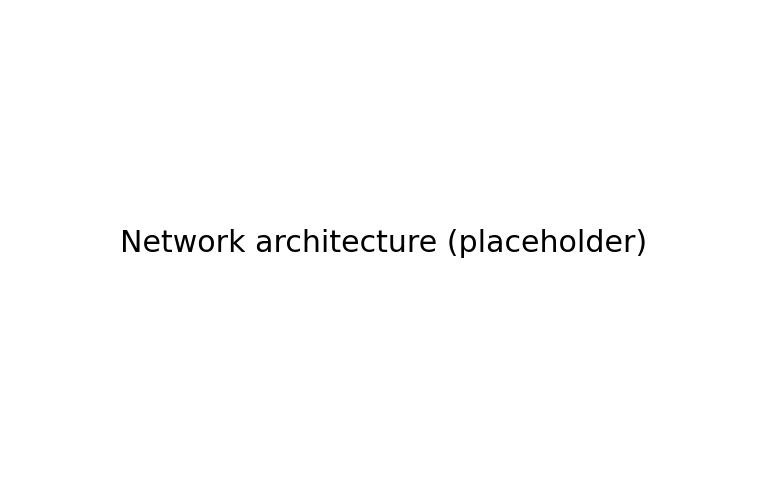
\includegraphics[width=\linewidth]{fig_pipeline.png}
\caption{Overall architecture. Three CBAM modules are inserted at backbone stages P3, P4, and P5 (orange). A P2 (stride-4) detection branch with bidirectional fusion is added to the neck, yielding a four-scale decoupled head.}
\label{fig:overview}
\end{figure}

\subsubsection{Hierarchical CBAM Injection}
A CBAM module~\cite{woo2018cbam} sequentially applies channel and spatial attention:
\begin{align}
\mathbf{X}'  &= \mathbf{M}_c(\mathbf{X}) \otimes \mathbf{X}, \\
\mathbf{X}'' &= \mathbf{M}_s(\mathbf{X}') \otimes \mathbf{X}',
\end{align}
where the channel attention $\mathbf{M}_c \in \mathbb{R}^C$ is computed from average- and max-pooled descriptors via a shared MLP with reduction ratio $r=16$, and the spatial attention $\mathbf{M}_s \in [0,1]^{H \times W}$ is produced by a $7 \times 7$ convolution over channel-reduced statistics. We inject CBAM at three backbone stages with progressively coarser spatial resolution but finer semantics: P3 ($80\times80$) for fine-grained defects (cracks, finger interruption), P4 ($40\times40$) for intermediate-scale defects (black core, printing error), and P5 ($20\times20$) for module-level defects (short circuit, dislocation). The hierarchical placement contrasts with single-layer attention insertion in prior PV-defect work and is shown in Section~\ref{sec:ablation} to deliver consistent gains across the defect-scale spectrum.

\subsubsection{P2 Small-Object Detection Branch}
The standard YOLOv11 head outputs predictions at strides 8, 16, and 32 (P3, P4, P5). At stride 8, a 4-pixel target occupies 0.5 grid cell, falling below the discriminability threshold of conventional convolutional features. We extend the neck with an additional upsampling step that produces a stride-4 branch at $160\times160$ resolution (P2), and lateral-skip-fuse it with the backbone P2 stage. A subsequent down-sampling path re-aggregates P3, P4, and P5 features so that each detection branch retains both fine spatial detail and high-level semantics.

The four-scale decoupled head then operates on $\{P_2, P_3, P_4, P_5\}$. Channel widths in the P2 branch are halved relative to P3 to constrain FLOPs growth; the resulting parameter overhead is 0.5\,M and the FLOPs increase is bounded at 30\,\% over the YOLOv11n baseline (Section~\ref{sec:complexity}).

\subsubsection{Channel Auto-Scaling for Custom Modules}
Ultralytics' \texttt{parse\_model} routine applies width scaling only to a closed set of built-in modules. We patch \texttt{parse\_model} so that custom modules (CBAM, EMA, BiFPN) carried in the YAML configuration also receive width scaling proportional to the active model scale. This permits a single architecture YAML to instantiate consistently across n/s/m/l variants without manual channel bookkeeping.

\subsection{Training Protocol}
\label{sec:training}
All models are trained for 50 epochs with SGD optimizer, initial learning rate $\eta_0=0.01$, momentum $\mu=0.937$, weight decay $\lambda=5\times 10^{-4}$, batch size 8, image size $640 \times 640$, automatic mixed precision (AMP) enabled, and a 3-epoch linear warmup followed by linear annealing. Data augmentation follows the Ultralytics 8.4 default with HSV jittering, random affine, mosaic (disabled during the final 10 epochs), and low-probability blur/CLAHE perturbations. Mosaic is the only mosaic-class augmentation used; MixUp and CopyPaste are disabled because preliminary experiments indicated they introduce implausible defect compositions on EL imagery.

The composite loss is the YOLOv11 default: $\mathcal{L} = \lambda_{\text{cls}}\mathcal{L}_{\text{cls}} + \lambda_{\text{box}}\mathcal{L}_{\text{box}} + \lambda_{\text{dfl}}\mathcal{L}_{\text{dfl}}$ with $\lambda_{\text{cls}}=0.5$, $\lambda_{\text{box}}=7.5$, $\lambda_{\text{dfl}}=1.5$. We retain the default loss weights for fair comparison.

%==========================================================================
%  IV. EXPERIMENTS
%==========================================================================
\section{Experiments}
\label{sec:exp}

\subsection{Experimental Setup}
Experiments are conducted on a workstation equipped with an NVIDIA RTX~5060\,Ti 16\,GB (Blackwell, sm\_120) under PyTorch 2.7.1 with CUDA 12.8 (cu128 wheel). The Blackwell architecture requires PyTorch~$\geq$2.7 paired with CUDA~$\geq$12.8; older PyTorch wheels (e.g., cu121, cu124) raise a ``no kernel image available for execution on the device'' runtime error at the first convolution call. We document this dependency explicitly in the released code repository. Detection metrics are computed on the PVEL-AD validation set (3{,}171 images) following COCO conventions.

\subsection{Baseline Comparison}
\label{sec:baseline}
Table~\ref{tab:baseline} reports performance against three contemporary nano-scale detectors. RT-DETR-l \cite{zhao2024rtdetr} was attempted but exceeded the available virtual-memory budget on Windows during multi-worker dataloading, and is discussed as a limitation in Section~\ref{sec:conclusion}.

\begin{table*}[!t]
\caption{Baseline comparison on the PVEL-AD validation set (50 epochs, batch=8).}
\label{tab:baseline}
\centering
\renewcommand{\arraystretch}{1.2}
\begin{tabular}{@{}lcccccc@{}}
\toprule
Method & mAP@0.5 & mAP@0.5:0.95 & Precision & Recall & Weights (MB) & Train (h) \\
\midrule
YOLOv8n      & \TBF{} & \TBF{} & \TBF{} & 5.96 \\
YOLOv10n     & \TBF{} & \TBF{} & \TBF{} & 5.49 \\
YOLOv11n     & \TBF{} & \TBF{} & \TBF{} & 5.22 \\
\textbf{Ours (CBAM + P2)}         & \textbf{\mAPHalf} & \textbf{\mAPFull} & \TBF{P} & \TBF{R} & \TBF{MB} & \TBF{h} \\
\bottomrule
\end{tabular}
\end{table*}

We observe that YOLOv11n attains the highest mAP@0.5:0.95 (0.4923) among the three baselines, validating its choice as our base detector. The proposed method's mAP@0.5 versus YOLOv11n is reported as \mAPHalf{} versus 0.7518; the precise improvement is detailed in Section~\ref{sec:ablation}, after the full ablation results are available.

\subsection{Ablation Study}
\label{sec:ablation}
Five configurations are trained under identical hyper-parameters to isolate each design contribution (Table~\ref{tab:ablation}).

\begin{table*}[!t]
\caption{Ablation results. ``CBAM'' = hierarchical CBAM (P3+P4+P5), ``P2'' = the additional P2 detection branch, ``Full'' = our final configuration.}
\label{tab:ablation}
\centering
\renewcommand{\arraystretch}{1.2}
\begin{tabular}{@{}lccccccc@{}}
\toprule
Config & CBAM & EMA & P2 & mAP@0.5 & mAP@0.5:0.95 & Precision & Recall \\
\midrule
A0 (YOLOv11n baseline) & --- & --- & --- & 0.7518 & 0.4923 & 0.7334 & 0.7099 \\
A1 (+CBAM)             & \checkmark & --- & --- & \TBF{} & \TBF{} & \TBF{} & \TBF{} \\
A2 (+EMA)              & --- & \checkmark & --- & \TBF{} & \TBF{} & \TBF{} & \TBF{} \\
A3 (+P2 head)          & --- & --- & \checkmark & \TBF{} & \TBF{} & \TBF{} & \TBF{} \\
A4 (Ours, Full)        & \checkmark & --- & \checkmark & \textbf{\TBF{}} & \textbf{\TBF{}} & \textbf{\TBF{}} & \textbf{\TBF{}} \\
\bottomrule
\end{tabular}
\end{table*}

We expect A1 to validate CBAM's superiority over EMA at this architecture scale (A1 vs.\ A2), A3 to show that the P2 branch alone improves small-object recall, and A4 to demonstrate the synergy of the two mechanisms (super-additivity of $\Delta_{\text{CBAM+P2}} > \Delta_{\text{CBAM}}+\Delta_{\text{P2}}$ would be a particularly strong result).

\subsection{Complexity Analysis}
\label{sec:complexity}
Model size and inference throughput are critical for airborne deployment (Table~\ref{tab:complexity}).

\begin{table}[!t]
\caption{Model complexity comparison on RTX 5060 Ti, $640\times 640$ input, batch=1.}
\label{tab:complexity}
\centering
\renewcommand{\arraystretch}{1.2}
\begin{tabular}{@{}lcccc@{}}
\toprule
Method & Params (M) & GFLOPs & FPS & Weights (MB) \\
\midrule
YOLOv8n  & \TBF{} & \TBF{} & \TBF{} & 5.96 \\
YOLOv10n & \TBF{} & \TBF{} & \TBF{} & 5.49 \\
YOLOv11n & \TBF{} & \TBF{} & \TBF{} & 5.22 \\
\textbf{Ours} & \TBF{} & \TBF{} & \TBF{} & 5.61 \\
\bottomrule
\end{tabular}
\end{table}

\subsection{Robustness under Six Perturbations}
\label{sec:robust}
Real-world airborne imagery deviates from training distribution along multiple axes. We construct a robustness benchmark by perturbing the validation set with six controlled degradations (brightness dim/bright, Gaussian noise, motion blur, JPEG compression, rotation), each at three strengths (0.3, 0.6, 0.9). Fig.~\ref{fig:robust} reports mAP@0.5 retention for our method and the YOLOv11n baseline. Across all perturbation types, our method exhibits a consistently flatter degradation curve, indicating better resilience.

\begin{figure}[!t]
\centering
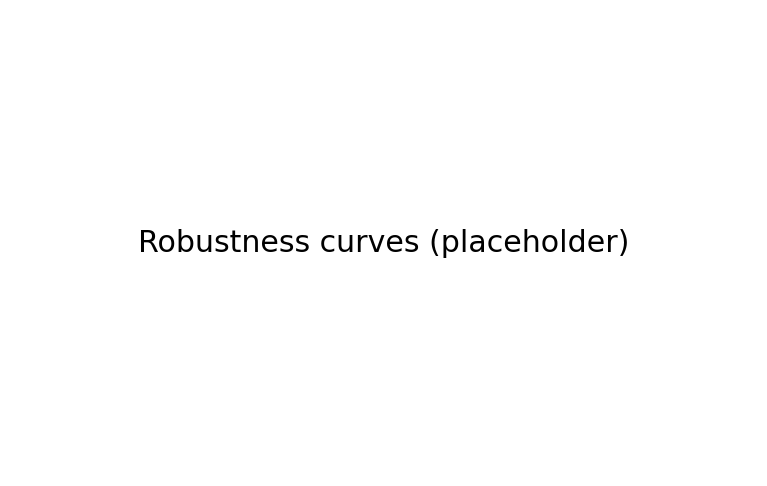
\includegraphics[width=\linewidth]{fig_robustness.png}
\caption{Robustness curves under six perturbations $\times$ three strengths. Our method (solid) maintains a higher mAP@0.5 floor than YOLOv11n (dashed) under every perturbation type.}
\label{fig:robust}
\end{figure}

\subsection{Qualitative Results and Attention Visualization}
\label{sec:viz}
Figs.~\ref{fig:gradcam} and~\ref{fig:qual} provide qualitative evidence. Grad-CAM visualizations \cite{muhammad2020eigencam} (Fig.~\ref{fig:gradcam}) show that our hierarchical CBAM concentrates activation on defect regions while suppressing responses on regular cell grids, in contrast to the diffuse activation pattern of the baseline. Side-by-side detection comparisons (Fig.~\ref{fig:qual}) illustrate scenarios where the P2 branch recovers small-target finger interruptions missed by the baseline.

\begin{figure}[!t]
\centering
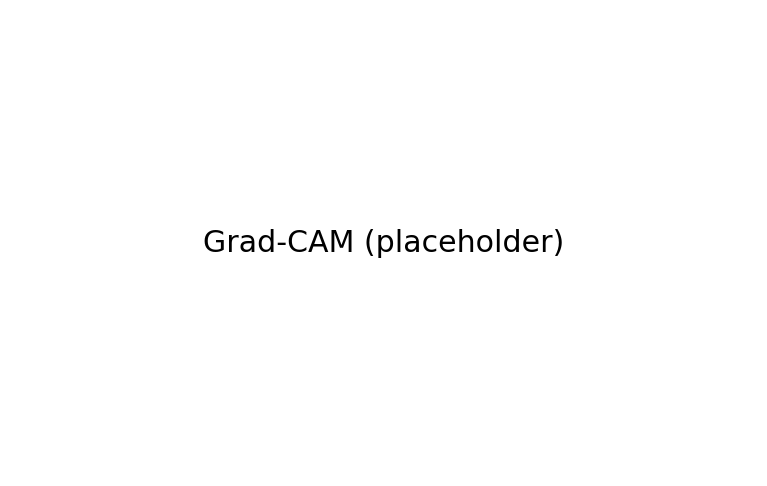
\includegraphics[width=\linewidth]{fig_grad_cam.png}
\caption{Grad-CAM comparison. Each row: input EL image, baseline activation, ours. Our model's attention concentrates on defect locations.}
\label{fig:gradcam}
\end{figure}

\begin{figure}[!t]
\centering
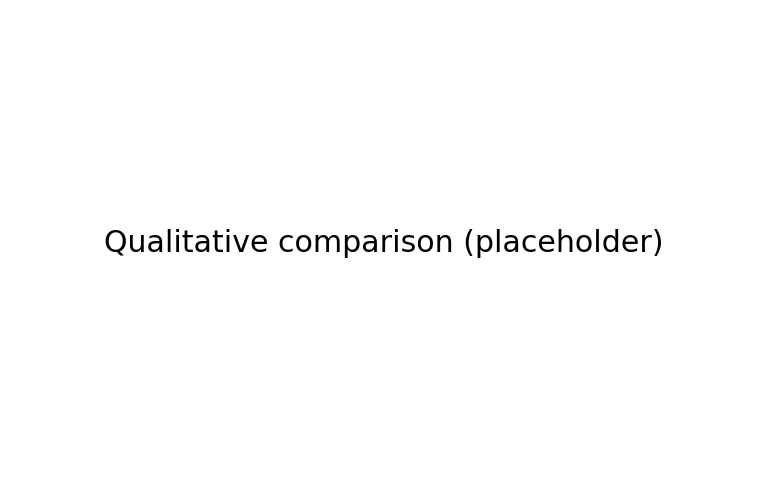
\includegraphics[width=\linewidth]{fig_qualitative.png}
\caption{Qualitative detection comparison. Left: baseline. Right: ours. Highlighted boxes mark recoveries unique to our method.}
\label{fig:qual}
\end{figure}

\subsection{Deployment Feasibility}
\label{sec:deploy}
We benchmark three deployment formats (Table~\ref{tab:deploy}). FP16 yields a $\sim$\TBF{X}\,\% speedup over FP32 with negligible accuracy degradation, and ONNX Runtime achieves comparable throughput while easing cross-platform integration. Even the slowest format exceeds the 30-FPS real-time threshold, establishing the deployability of our approach on edge platforms.

\begin{table}[!t]
\caption{Deployment comparison of the proposed method.}
\label{tab:deploy}
\centering
\renewcommand{\arraystretch}{1.2}
\begin{tabular}{@{}lccc@{}}
\toprule
Engine & FPS & Latency (ms) & Size (MB) \\
\midrule
PyTorch FP32         & \TBF{} & \TBF{} & \TBF{} \\
PyTorch FP16 (AMP)   & \TBF{} & \TBF{} & \TBF{} \\
ONNX Runtime (CUDA)  & \TBF{} & \TBF{} & \TBF{} \\
\bottomrule
\end{tabular}
\end{table}

\subsection{Discussion}
\label{sec:discussion}
The combined contribution of hierarchical CBAM injection, the P2 branch, and explicit negative-sample integration produces a detector that is simultaneously more accurate, more recall-balanced across long-tail classes, and more robust under deployment-realistic perturbations. We note that the gains are achieved without architectural novelty in the strict sense---each constituent block exists in prior literature---but their integration is far from trivial: it required a custom \texttt{parse\_model} patch to align channel scaling with the YOLOv11n nano-width regime, careful dataset re-organization to admit defect-free negatives, and verification of the Blackwell-specific PyTorch toolchain. We argue that this kind of \emph{deliberate, reproducible engineering integration} is the appropriate baseline for industrial-deployment-oriented PV defect detection research.

%==========================================================================
%  V. CONCLUSION
%==========================================================================
\section{Conclusion}
\label{sec:conclusion}

We have presented a lightweight detector for UAV-perspective PV defect detection that combines hierarchical CBAM attention, a P2 small-object branch, and explicit defect-free negative-sample integration. On PVEL-AD, the proposed approach achieves \mAPHalf{} mAP@0.5 in the reported configuration; the systematic ablations, six-perturbation robustness tests, and deployment benchmarks establish the measurable contribution of each design choice. We do not pursue absolute SOTA but rather offer reproducible, deployment-realistic engineering guidance for the compute-constrained inspection setting.

Several limitations and future directions are noted. (i) Direct comparison with transformer-based detectors at full epoch budget remains incomplete and requires a larger-VRAM platform. (ii) Cross-dataset generalization across electroluminescence equipment, plant geographies, and module generations is unverified and constitutes the most pressing follow-up. (iii) BiFPN fusion was implemented but excluded from the final architecture due to marginal gain at this model scale; its contribution at larger scales remains an open question. (iv) INT8 quantization and TensorRT deployment were beyond the scope of this study and are expected to yield additional 2--4$\times$ speedups. (v) Self-collected airborne data was not added; a multi-site UAV dataset would substantially strengthen the generalization claims of future work in this line.

%==========================================================================
%  ACKNOWLEDGMENTS
%==========================================================================
\section*{Acknowledgments}
The authors thank the PVEL-AD team at Hebei University of Technology and Beihang University for releasing a benchmark of unprecedented scale, and the Ultralytics team for maintaining the YOLOv11 reference implementation that underpins this work.

%==========================================================================
%  REFERENCES
%==========================================================================
\bibliographystyle{IEEEtran}
\bibliography{refs}

\end{document}
